\subsection{Extending the Naive-dynamic (ND) approach to Parallel Leiden algorithm}

Our earlier work \cite{sahu2024dflouvain} presented a parallel version of the Naive-dynamic (ND) approach, which utilizes the weighted degrees of vertices and the total edge weights of communities as auxiliary information, as shown in Figure \ref{fig:about-auxiliary}. In this report, we extend it to Parallel Leiden algorithm \cite{sahu2023gveleiden}. The psuedocode for this is given in Algorithm \ref{alg:naive}, and its explanation in Section \ref{sec:our-naive}.

\begin{figure}[hbtp]
  \centering
  \subfigure{
    \label{fig:about-auxiliary--with}
    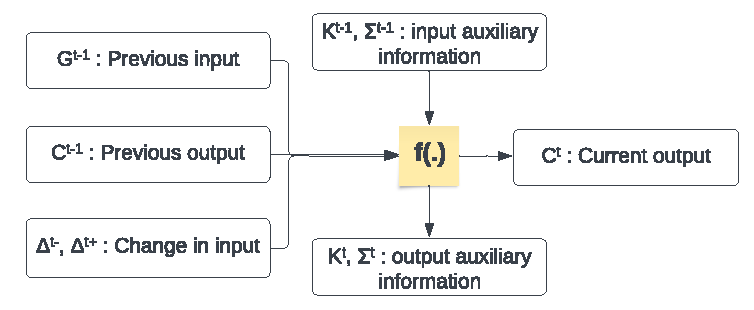
\includegraphics[width=0.98\linewidth]{out/about-auxiliary-with.pdf}
  } \\[-2ex]
  \caption{A dynamic community detection algorithm $f(.)$ takes as input the previous graph $G^{t-1}$, community memberships $C^{t-1}$, and the batch update $\Delta^{t-}$, $\Delta^{t+}$, and produces the updated community memberships $C^t$. However, it may also consider additional information such as the weighted degrees of vertices $K^{t-1}$ and the total edge weights of communities $\Sigma^{t-1}$ as auxiliary information, and yield updated auxiliary information $K^t$, $\Sigma^t$ \cite{sahu2024dflouvain}.}
  \label{fig:about-auxiliary}
\end{figure}





\subsection{Extending the Delta-screening (DS) approach to Parallel Leiden algorithm}

The Delta-screening (DS) approach proposed by Zarayeneh et al. \cite{com-zarayeneh21} is sequential. Our previous work \cite{sahu2024dflouvain} adapted it into an efficient parallel algorithm, which employed per-thread collision-free hash tables, and leveraged the weighted degrees of vertices and the total edge weights of communities as auxiliary information. Here, we extend this approach to Parallel Leiden algorithm \cite{sahu2023gveleiden}, by processing only the marked vertices during the local-moving phase, but processing all vertices during the refinement phase of the first pass\ignore{of the Leiden algorithm}. The psuedocode for this is in Algorithm \ref{alg:delta}, with a detailed explanation of the psuedocode given in Section \ref{sec:our-delta}.




\subsection{Extending the Dynamic Frontier (DF) approach to Parallel Leiden algorithm}

Our prior study \cite{sahu2024dflouvain} presented a parallel implementation of the Dynamic Frontier (DF) approach, which, as above, utilized per-thread collision-free hash tables and capitalized on the weighted degrees of vertices and the total edge weights of communities as auxiliary information. In this work, we expand upon this, by applying it to Parallel Leiden\ignore{\cite{sahu2023gveleiden}} instead. The pseudocode for this is outlined in Algorithm \ref{alg:delta}, accompanied by an explanation provided in Section \ref{sec:our-delta}. Similar to our DS Leiden counterpart, it processes the (incrementally) marked vertices during the local-moving phase, but operates on all vertices during the refinement phase\ignore{(of the first pass)} of Leiden algorithm.

\begin{figure}[!hbt]
  \centering
  \subfigure{
    \label{fig:optimize-subrefine--8020}
    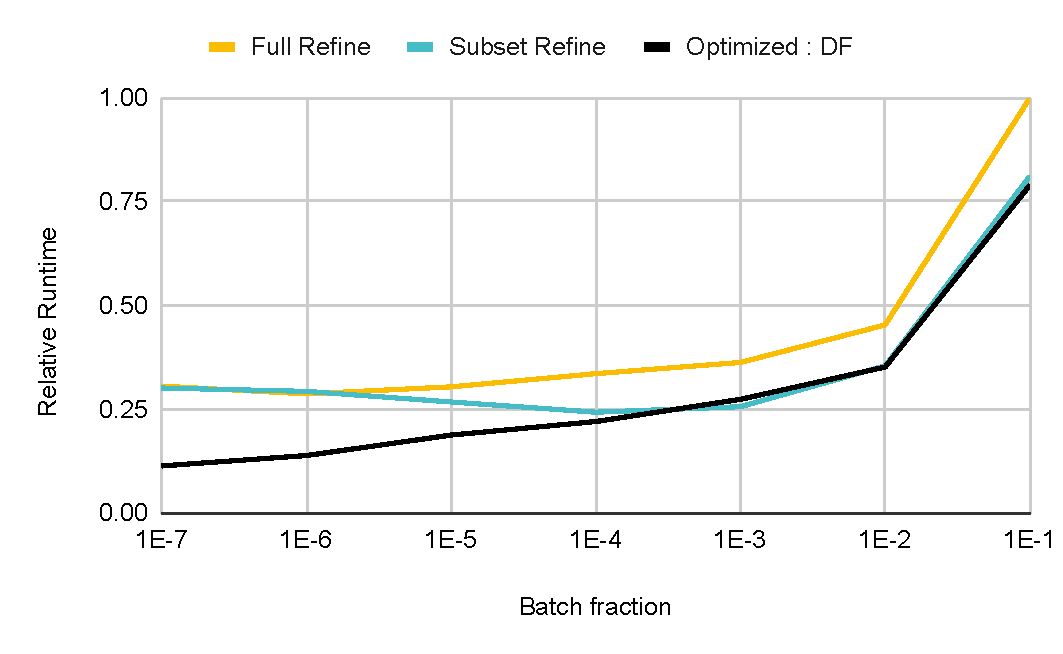
\includegraphics[width=0.98\linewidth]{out/optimize-subrefine-8020.pdf}
  } \\[-2ex]
  \caption{Mean Runtime and Modularity of communities obtained with our multicore implementation of \textit{Static}, \textit{Naive-dynamic (ND)}, \textit{Delta-screening (DS)}, and \textit{Dynamic Frontier (DF)} Leiden on real-world dynamic graphs, using batch updates of size $10^{-5}|E_T|$ to $10^{-3}|E_T|$. Here, (a) and (b) display the overall runtime and modularity across all temporal graphs, while (c) and (d) display the runtime and modularity for each individual graph. In (a), the speedup of each approach relative to Static Leiden is labeled.}
  \label{fig:optimize-subrefine}
\end{figure}

\begin{figure}[!hbt]
  \centering
  \subfigure[Relative runtimes on uniformly random batch updates of size $10^{-7}|E|$]{
    \label{fig:aggregation-adjust-chunksize--batch7}
    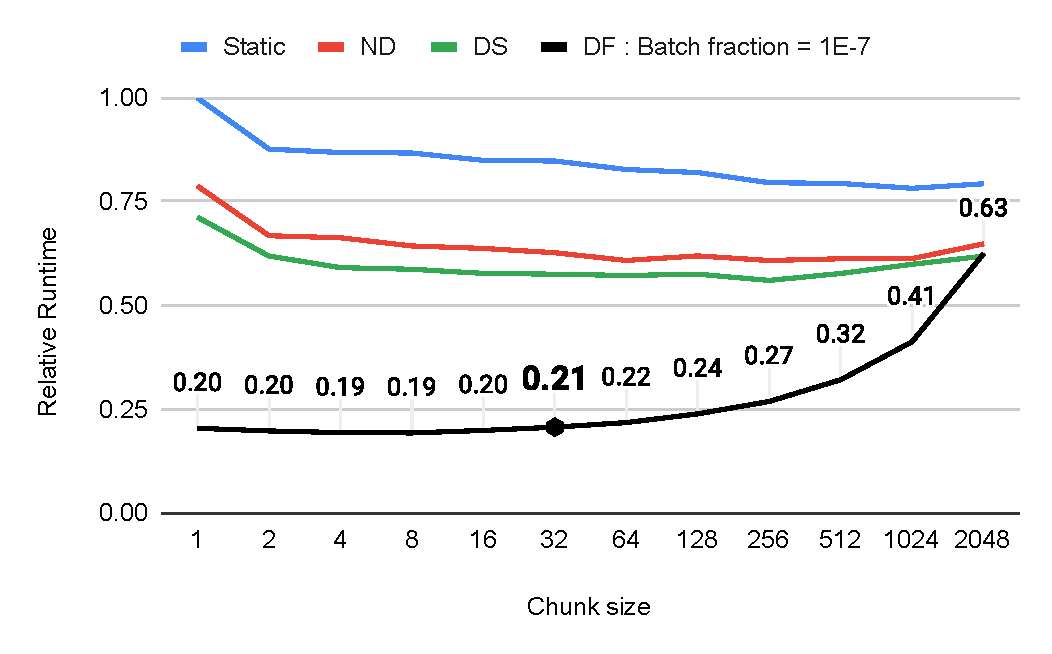
\includegraphics[width=0.98\linewidth]{out/aggregation-adjust-chunksize7.pdf}
  }
  \subfigure[Relative runtimes on uniformly random batch updates of size $10^{-5}|E|$]{
    \label{fig:aggregation-adjust-chunksize--batch5}
    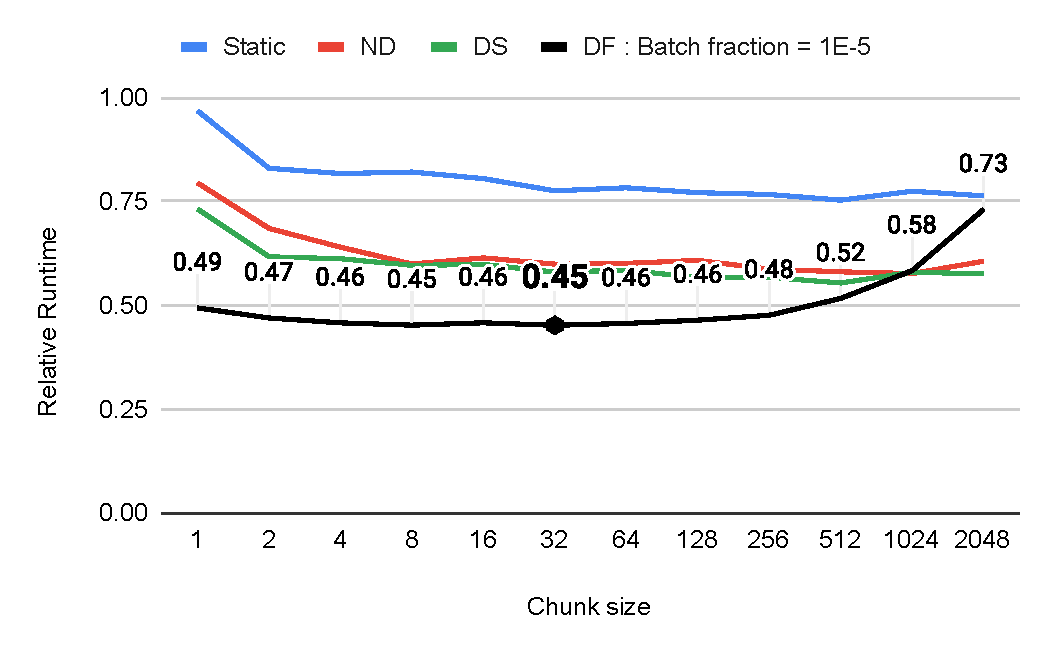
\includegraphics[width=0.98\linewidth]{out/aggregation-adjust-chunksize5.pdf}
  }
  \subfigure[Relative runtimes on uniformly random batch updates of size $10^{-3}|E|$]{
    \label{fig:aggregation-adjust-chunksize--batch3}
    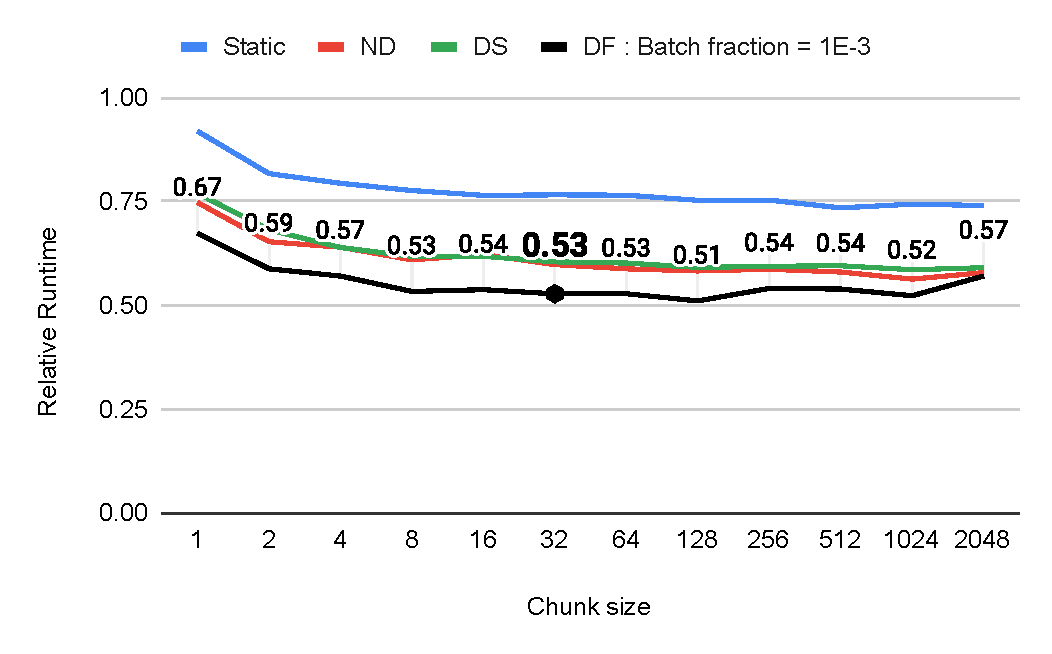
\includegraphics[width=0.98\linewidth]{out/aggregation-adjust-chunksize3.pdf}
  } \\[-1ex]
  \caption{Relative Runtime of \textit{Static}, \textit{Naive-dynamic (ND)}, \textit{Delta-screening (DS)}, and \textit{Dynamic Frontier (DF)} Leiden, with varying dynamic schedule chunk size (OpenMP), for aggregation phase of the Leiden algorithm. These tests were conducted on large graphs, with batch updates randomly generated at sizes of $10^{-7}|E|$, $10^{-5}|E|$, and $10^{-3}|E|$. The results suggest that a chunk size of $32$ is optimal (highlighted).}
  \label{fig:aggregation-adjust-chunksize}
\end{figure}

